%%%%%%%%%%%%%%%%%%%%%%%%%%%%%%%%%%%%%%%%%%%%%%%%%%%%%%%%%%%%%%%%%%%%%%%%
\chapter{Soluzioni degli esercizi del Capitolo \ref{cap:basi}}
%%%%%%%%%%%%%%%%%%%%%%%%%%%%%%%%%%%%%%%%%%%%%%%%%%%%%%%%%%%%%%%%%%%%%%%%

%%%%%%%%%%%%%%%%%%%%%%%%%%%%%%%%%%%%%%%%%%%%%%%%%%%%%%%%%%%%%%%%%%%%%%%%
\section*{Esercizio \ref{ex:02-relaSOmega}}
\addcontentsline{toc}{section}{Esercizio \ref{ex:02-relaSOmega}}
%%%%%%%%%%%%%%%%%%%%%%%%%%%%%%%%%%%%%%%%%%%%%%%%%%%%%%%%%%%%%%%%%%%%%%%%

Data la natura additiva di $S$ e moltiplicativa di $\Omega$ la funzione $f$ deve necessariamente soddisfare la relazione
\be
\label{ans2:o1o2}
f(\Omega_1\Omega_2) = f(\Omega_1) + f(\Omega_2)
\ee
Differenziando la precedente sia rispetto a $\Omega_1$ sia rispetto a $\Omega_2$ otteniamo le due equazioni
\be
\Omega_2 f'(\Omega_1\Omega_2) = f'(\Omega_1) \quad\quad
\Omega_1 f'(\Omega_1\Omega_2) = f'(\Omega_2)
\ee
Dividendo l'una per l'altra otteniamo
\be
\Omega_1 f'(\Omega_1) = \Omega_2 f'(\Omega_2)
\ee
Ma il termine a sinistra dell'equazione è indipendente da $\Omega_2$, mentre il termine a destra è indipendente da $\Omega_1$. Poiché sono uguali, entrambi i termini devono necessariamente essere una costante $k$ indipendente sia da $\Omega_1$ sia da $\Omega_2$. Abbiamo dunque
\be
f'(\Omega) = \dfrac{k}{\Omega}
\ee
e cioè
\be
f(\Omega) = k\ln(\Omega) + c
\ee
in cui $c$ è una costante di integrazione. Inserendo l'ultima equazione nella (\ref{ans2:o1o2}) vediamo subito che $c=0$.

%%%%%%%%%%%%%%%%%%%%%%%%%%%%%%%%%%%%%%%%%%%%%%%%%%%%%%%%%%%%%%%%%%%%%%%%
\section*{Esercizio \ref{ex:02-sfere}}
\addcontentsline{toc}{section}{Esercizio \ref{ex:02-sfere}}
%%%%%%%%%%%%%%%%%%%%%%%%%%%%%%%%%%%%%%%%%%%%%%%%%%%%%%%%%%%%%%%%%%%%%%%%

Costruiamo il nostro sistema aggiungendo una particella alla volta. Il primo atomo, trascurando effetti di bordo, avrà a disposizione un volume $V$. Per il secondo atomo occorre considerare il volume già occupato dal primo; avrà quindi a disposizione un volume pari a $(V-\alpha v_0)$, con $\alpha$ da determinare. Osservando la figura \ref{fig:02-sol-raggio2} si evince subito che il volume escluso è quello di una sfera di raggio $2r$, e cioè $8v_0$. 
%%%%%%%%%%%%%%%%%%%%%%%%%%%%%%%%%%%%%%%%%%%%%%%%%%%%%%%%%%%%%%%%%%%%%%
\begin{figure}[!ht]
\centering
  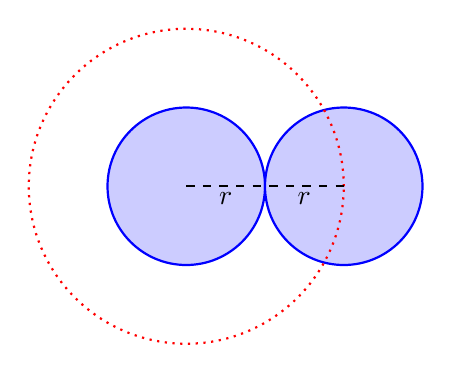
\begin{tikzpicture}[scale=0.5]
  \draw[thick,blue,fill=blue!20] (0,0) circle (2);
  \draw[thick,blue,fill=blue!20] (4,0) circle (2);
  \draw[thick,red,dotted] (0,0) circle (4);
  \draw[thick,dashed] (0,0)--(4,0);
  \draw (1,-0.3) node{$r$};
  \draw (3,-0.3) node{$r$};
\end{tikzpicture}


  \caption{Effetti di volume escluso.}
  \label{fig:02-sol-raggio2}
\end{figure}
%%%%%%%%%%%%%%%%%%%%%%%%%%%%%%%%%%%%%%%%%%%%%%%%%%%%%%%%%%%%%%%%%%%%%%
Dunque $\alpha = 8$. Per la dipendenza del numero dei microstati dal volume otteniamo dunque subito
\bea
\Omega &\propto& V(V-8v_0)(V-16v_0)\cdots(V-8kv_0)\cdots(V-8(N-1)v_0) \nonumber\\
	   &=& \prod_{k=0}^{N-1}(V-8kv_0)
\eea
Abbiamo quindi, con $C$ indipendente dal volume $V$, 
\bea
\ln\Omega &=& \sum_{k=0}^{N-1}\ln(V-8kv_0) + C = \sum_{k=0}^{N-1}\ln[V(1-8kv_0/V)] + C \nonumber\\
&\simeq& N\ln V -\frac{8v_0}{V}\sum_{k=0}^{N} k + C
\eea
in cui nell'ultimo passaggio abbiamo approssimato $N-1\simeq N$ e abbiamo espanso il logaritmo, $\ln(1+x) = x + \cdots$.
L'ultima sommatoria nella precedente vale $N(N+1)/2$, che approssimiamo con $N^2/2$. Otteniamo quindi, per l'entropia,
\be
S = kN\left\{ \ln V - \frac{4Nv_0}{V} \right\} + kC
\ee
Utilizziamo ora la formula
\be
\frac{P}{T} = \dparc{S}{V}{N,E}
\ee
per ottenere
\be
P = \frac{NkT}{V}\left\{ 1 + \frac{4Nv_0}{V} \right\}
\ee
Troviamo quindi un volume efficace pari a
\be
V_{\textrm{eff}} = \frac{V}{1+4Nv_0/V} \simeq V\left\{ 1 - \frac{4Nv_0}{V} \right\} = V-4Nv_0
\ee
che è esattamente il risultato che ci eravamo proposti di dimostrare.

%%%%%%%%%%%%%%%%%%%%%%%%%%%%%%%%%%%%%%%%%%%%%%%%%%%%%%%%%%%%%%%%%%%%%%%%
\section*{Esercizio \ref{ex:02-Saddit}}
\addcontentsline{toc}{section}{Esercizio \ref{ex:02-Saddit}}
%%%%%%%%%%%%%%%%%%%%%%%%%%%%%%%%%%%%%%%%%%%%%%%%%%%%%%%%%%%%%%%%%%%%%%%%

Se $S$ è estensiva sappiamo che dev'essere direttamente proporzionale a $N$, cioè
\be
S(E,N,V) = Nf(E,V)
\ee
A questo punto però la rimanente funzione $f(E,V)$ dev'essere in realtà funzione di $(E/N,V/N) \equiv (\eps, v)$:
\be
S(E,N,V) = Nf(\eps, v)
\ee
Abbiamo dunque:
\bea
N\dparc{S}{N}{E,V} &=& N\left[
f(\eps,v) + N\dparc{f}{\eps}{v}\dpar{\eps}{N} + N\dparc{f}{v}{\eps}\dpar{v}{N}
\right] \nonumber \\
&=& N\left[
f(\eps,v) - \dparc{f}{\eps}{v}\dfrac{E}{N} - \dparc{f}{v}{\eps}\dfrac{V}{N}
\right] \nonumber \\
E\dparc{S}{E}{N,V} &=& NE\dparc{f}{\eps}{v}\dpar{\eps}{N} = E\dparc{f}{\eps}{v} \nonumber \\
V\dparc{S}{V}{E,V} &=& NV\dparc{f}{v}{\eps}\dpar{v}{N} = V\dparc{f}{v}{\eps}
\eea
Sommando le tre espressioni otteniamo il risultato cercato.

%%%%%%%%%%%%%%%%%%%%%%%%%%%%%%%%%%%%%%%%%%%%%%%%%%%%%%%%%%%%%%%%%%%%%%%%

\vskip 0.75cm
\begin{flushright}
{\em Ultimo aggiornamento del capitolo: 22.04.2017}
\end{flushright}
